\documentclass[14pt]{article}
\usepackage{mathtext}
\usepackage{bm}
\usepackage{amssymb}
\usepackage[T2A]{fontenc}
\usepackage[utf8]{inputenc}
\usepackage[russian]{babel}
\usepackage[
    left=30mm,
    top=20mm,
    right=10mm,
    bottom=20mm
]{geometry}
\usepackage{euscript}
\usepackage{graphicx}
\usepackage{amsmath,empheq,amsfonts, subcaption}
\graphicspath{ {./images/}{../images/} }

\begin{document}
\section{Детерминированные нейронные сети.}

Сначала напомним, что такое обычные(детерминированные) нейронные сети и как они обучаются.

Основная задача обычных искусственных нейронных сетей($ANN$) в том, чтобы аппроксимировать некоторую зависимость выхода $y$ от
 входа $x$: $y = \Phi(x)$.

Для простоты будем рассматривать обычные \textit{полносвязные} сети со входом $x$,
 скрытыми(промежуточными) состояниями слоёв $\bm{h_i}$, функциями активации $a_i(\cdot)$ и выходом $y$:
$$\bm{h_0} = \bm{x}$$
$$\bm{h_i} = a_i(\bm{W_i} \cdot h_{i-1} + \bm{b_i}), i = \overline{1...n}$$
$$\bm{h_n} = \widehat{y}$$
$$L = \mathcal{L}(\widehat{y}, y),$$ где $\mathcal{L}(\cdot, \cdot)$ - функция ошибки.

Обозначим параметры модели на $i$-ом слое $\bm{\theta_i} = (\bm{W_i}, \bm{b_i})$, а параметры всей модели через $\bm{\Theta} = \{\bm{\theta_i} :~i~=~\overline{1...n}\}$.
Чаще всего нейронные сети принято рассматривать, как вычислительный граф/граф вычислений.
 Такой подход удобен с инженерной точки зрения, поскольку позволяет воспользоваться инструментом автоматического
 дифференцирования, и используется во всех современных фреймоворках: PyTorch, TensorFlow и прочие.
 Граф вычислений является ациклическим ориентированным графом, составленным из вершин-переменных и вершин-операций(Рисунок 1).
\begin{figure}[ht]
    \subcaptionbox{\textit{Полносвязная} сеть в виде графа вычислений}{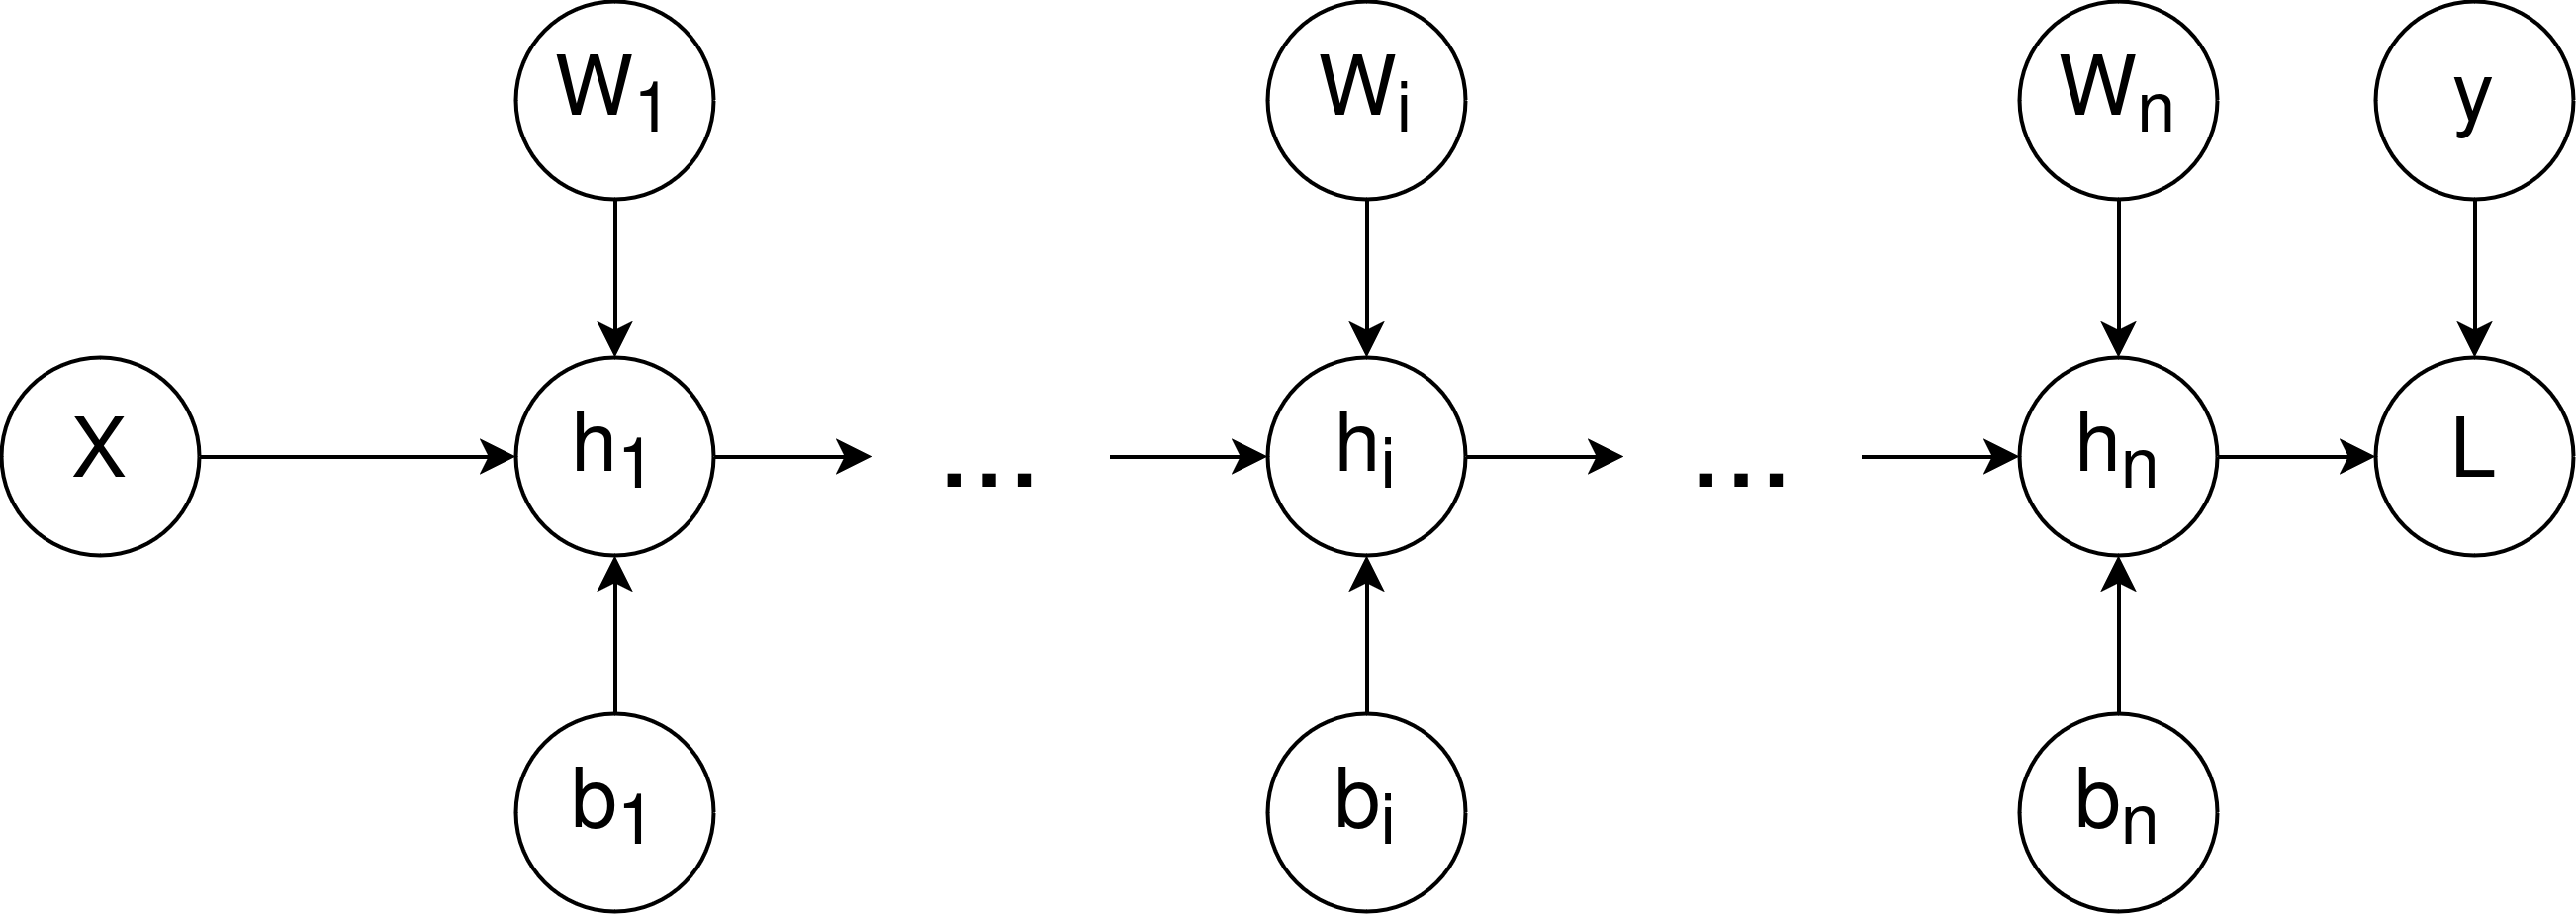
\includegraphics[width=8.5cm]{ANN.png}}
    \hfill
    \subcaptionbox{Обратное распространение ошибки по графу вычислений детерминированной полносвязной сети}{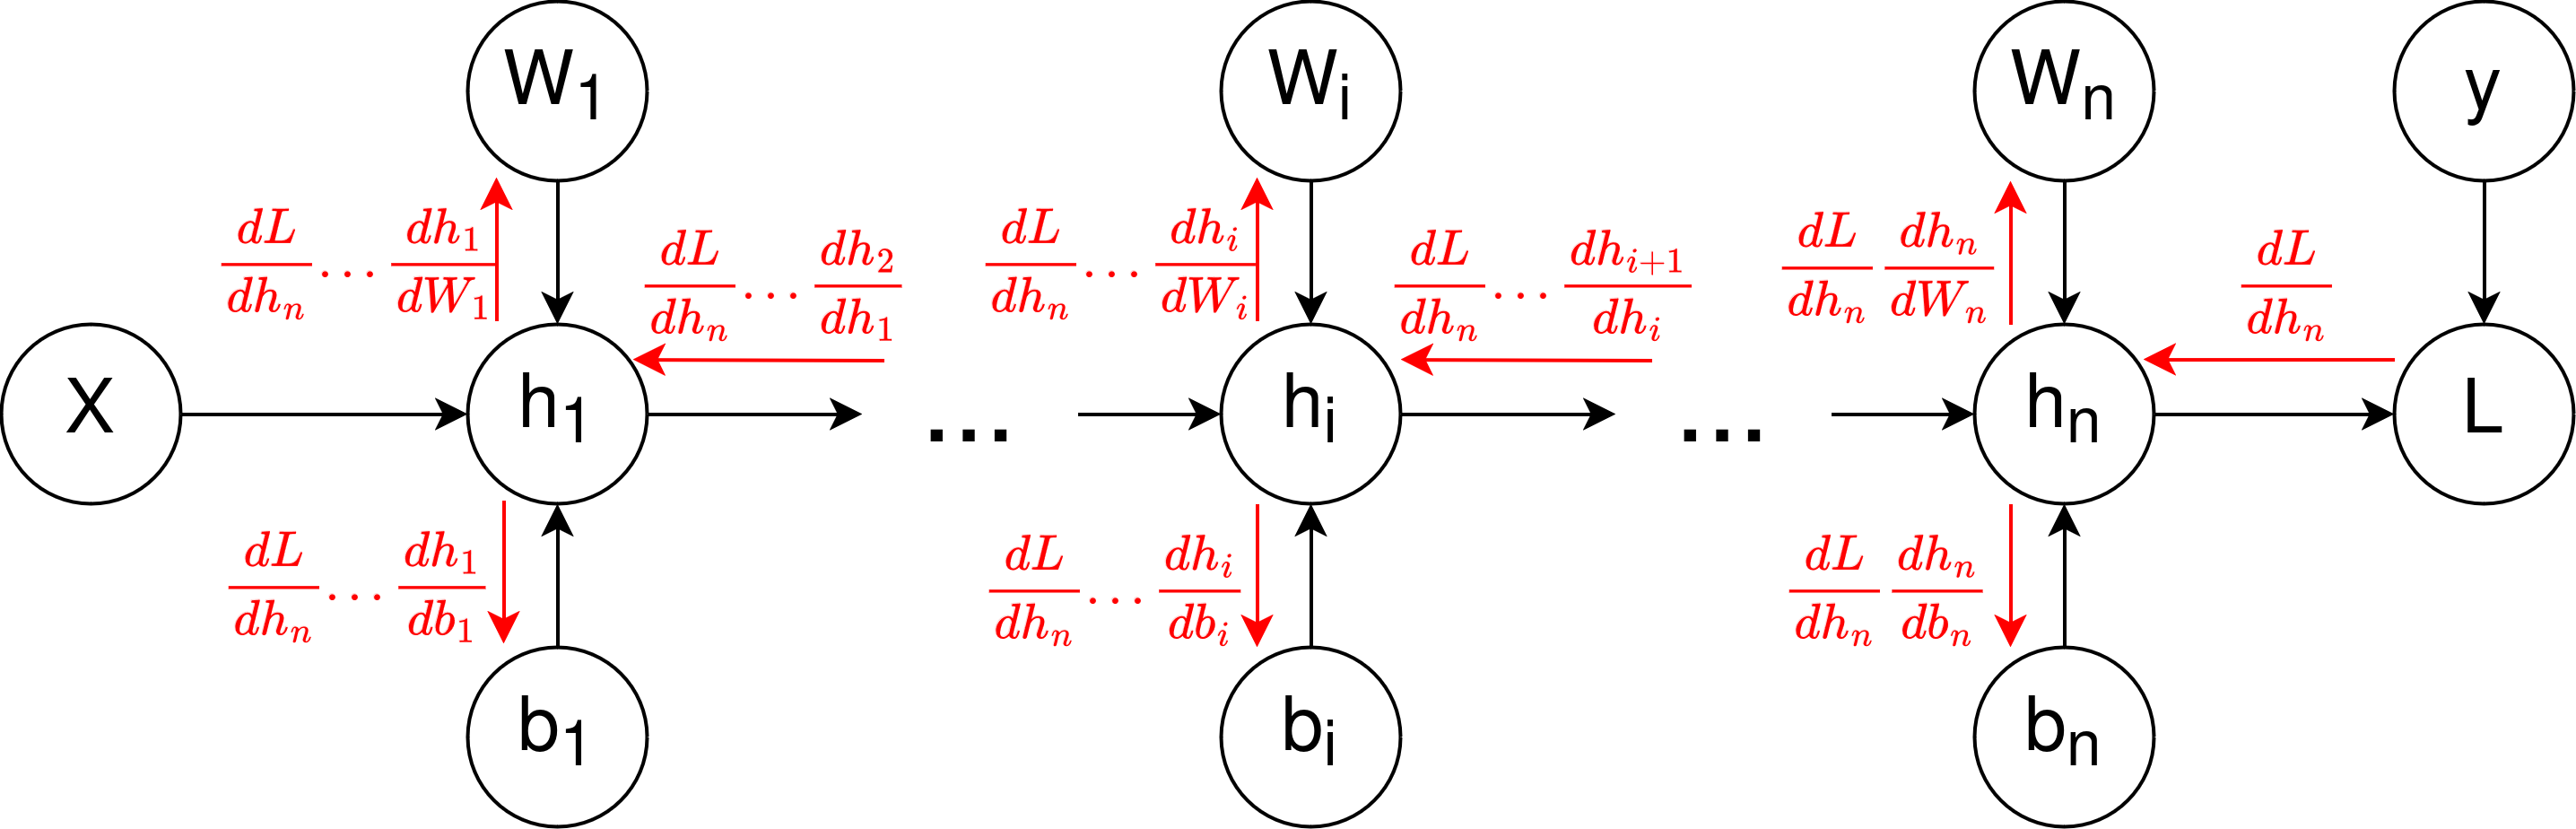
\includegraphics[width=8.5cm]{ANN_back_prop.png}}
\end{figure}


\end{document}
